\graphicspath{{chapters/images/08/}}

\chapter{Shotgun Metagenomics}

\section{Workflow}

\begin{figure}[!h]
\centering
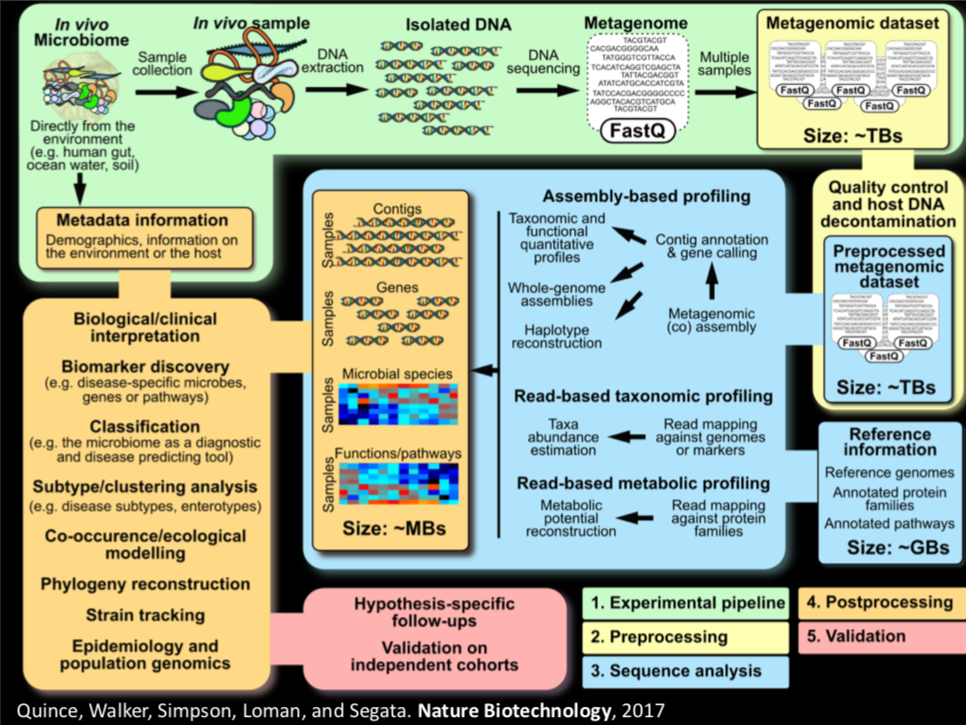
\includegraphics[width=0.9\textwidth]{Shotgun_workflow.png}
\caption{\label{fig:workflow}Shotgun metagenomics workflow}
\end{figure}

\begin{itemize}
\item \textbf{Experimental pipeline} → from sample collection to DNA sequencing.
\item \textbf{Preprocessing} → decontamination + quality control
\item \textbf{Mapping} or \textbf{assembling} (or both)
\item \textbf{Sequence analysis} → identification of microbial species + identification of present pathways/functions
\item \textbf{Post Processing} → integrate data with other information (where do the sample come from, healthy vs disease and other metadata)
\item \textbf{Validation} → follow-up experiments + independent replicates
\end{itemize}

\section{Comparison with the 16s sequencing}

\begin{tabular}{ | m{7cm}| m{7cm} | }
 \hline
 \multicolumn{2}{|c|}{\textbf{16S sequencing}} \\
 \hline
 \textbf{Pros} & \textbf{Cons} \\
 \hline
 Cost-effective & Non genome-wide \\
 Avoids non-bacterial contamination & Limited taxonomic resolution \\
 Can catch low-abundance bacteria & Not useful for pathogens profiling \\
 The output has reasonable size and complexity & Does not detect viruses or eukaryotes \\
 Mature software available to perform the computations & Several biases\\
 & Cross studies are difficult: the comparison is not possible due to biases \\
 \hline\hline
 \multicolumn{2}{|c|}{\textbf{Shotgun sequencing}} \\
 \hline
 \textbf{Pros} & \textbf{Cons} \\
 \hline
 Genome-wide: it is possible to retrieve information about all the genes present in the metagenome & Expensive (but costs are decreasing: right now the cost for the sequencing of one sample is ~100\$) \\
 High taxonomic resolution & DNA contamination are hard to remove \\
 Easy cross-study comparison thanks to the lack of biases & Low-abundance bacteria could be missed \\
 All domains of life can potentially be observed in the same study & Large dataset as output, that can be difficult to process (TBs of data) \\
 \hline
\end{tabular}

\section{Latest technology}

The cost of 100\$ for the sequencing of one sample refers to a sample size of 5Gb, that should be enough for shotgun metagenomics. More sequencing depth could be needed if you want to detect microbes with very low abundances, if you want to assemble as many genomes as possible and if there is a lot of contamination.

Shotgun metagenomics is possible with \textbf{Illumina Hiseq} technology, but the latest and most used technology nowadays is \textbf{Illumina NovaSeq}.

\section{Identification of microbes from Shotgun Metagenomics data: do we really need something fancy?}

\begin{figure}[!h]
\centering
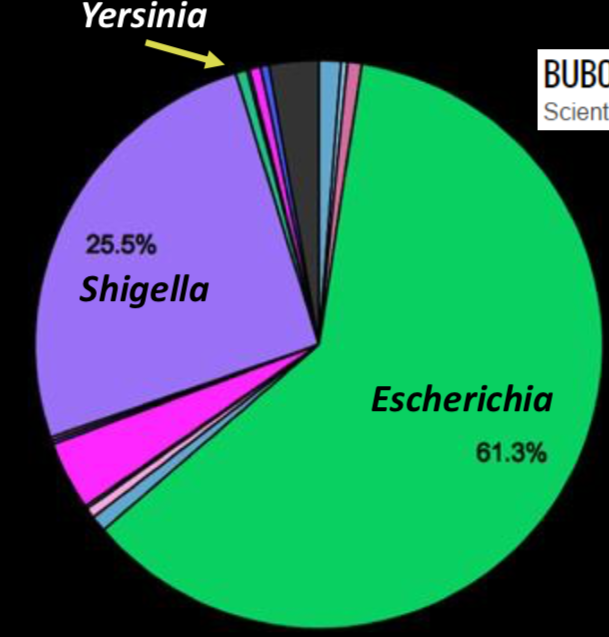
\includegraphics[width=0.4\textwidth]{Loman.png}
\caption{\label{fig:Loman}}
\end{figure}

 N.Loman studied why a simple alignment (with BowTie because with BLAST it is not feasible) is not enough to determine which microbial species are present in our samples. He took one \emph{E. coli} strain (K12), shredded its genome into 100 nts reads and classified these “reads” based on the best hit given by an alignment tool. Only 61\% of the reads were assigned to \emph{E. coli}. Even some Y.pestis resulted, probably because of some plasmid it has in common with \emph{E. coli} (\ref{fig:Loman}).
 
 With a similar approach, a study identified genes belonging to all sorts of organisms in samples taken in the New York City subway. \\

So yes, we need some fancy technique to solve this problem. The main \textbf{challenges} are:
\begin{itemize}
    \item How to obtain specie-specific resolution
    \item Computational feasibility
    \item Being able to detect both bacteria and archaea. Phages are also a problem since there is little reference
    \item Obtain relative abundances of organisms with different genome sizes: the problem is to obtain the organism abundance and not the DNA abundance
    \item Consistent detection confidence for all clades
    \item How to handle reads as short as 50 nts
    \item Detect organisms without a sequenced genome or still unknown species. 
\end{itemize}

\subsection{MetaPhlAn: unique marker genes for taxonomic profiling}

Solution brought to you by Segata with C. Huttenhower (\href{http://segatalab.cibio.unitn.it/tools/metaphlan/index.html}{reference})

\begin{figure}[!h]
\centering
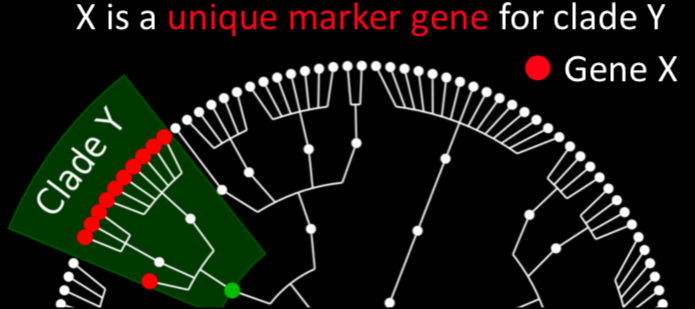
\includegraphics[width=0.7\textwidth]{markerGene.png}
\caption{\label{fig:markerGene}}
\end{figure}

The idea is to find a marker gene that uniquely characterizes a species(\ref{fig:markerGene}): it has to be present in all strains of a species and in no other species. These markers are then used to form taxonomic clades. The tool that generates the database is named \textbf{ChocoPhlAn}.

From a number of genomes, with ChocoPhlAn they created a database of marker genes of about 2 millions (400k are considered “most representative”) markers: the \textbf{MetaPhlAn} database. It contains about 200 markers per species. With the reduced size of this database compared with the whole genomes, it is possible to align the reads (first with BLAST, now they do it with BowTie2) directly on the markers database. 

\begin{figure}[!h]
\centering
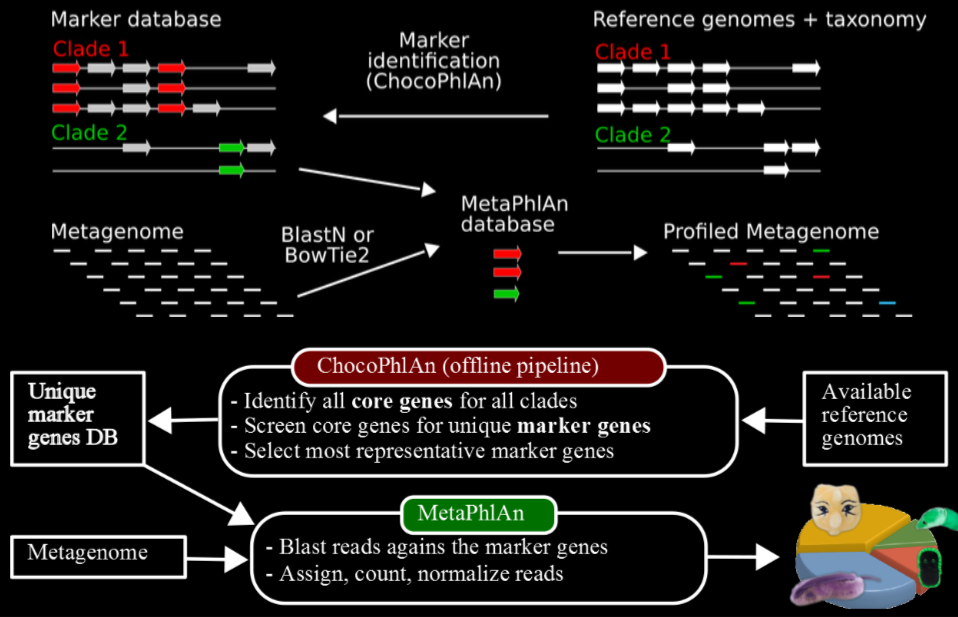
\includegraphics[width=0.95\textwidth]{MetaPhlAn.png}
\caption{\label{fig:metaphlan}MetaPhlAn overview}
\end{figure}

When they first created the marker genes database, they used 2887 genomes (and half of them were drafts) that belonged to 1222 species. The number of markers per species decreases with more sequenced genomes: the core genome tends to become smaller in size and noise is eliminated as more information is available. In the current version of BioBakery (the suite containing these tools) 1 million genomes are considered, of which about 200 000 are genome isolates and 800 000 are \textbf{MAGs} (Metagenomics-Assembled Genomes → putative genomes obtained from metagenomes).

MetaPhlAn computational performance can deal with about 200 000 reads per second and  can profile thousands of microbiomes in some hours. 

\textbf{Validation with synthetic metagenomes}: 10 well-known metagenomes were created and evaluated with MetaPhlAn to check if the results correspond to the actual species of microbes used to assemble the synthetic metagenome. Errors were also added in order to simulate sequencing noise. 

\textbf{Validation with biological methods}: comparison of the results with the ones obtained with 16S-based abundance estimation.

\subsubsection{The problem of the unknowns}

Microbial species that were never observed and do not have a marker in the database cannot be detected with this method.

The solution is to cluster together contigs obtained from the metagenome based on coverage, GC content, codon bias, and other possible features. Strict quality controls are then performed on these putative genomes: on the number of genes and the number of known single-copy genes in order to be sure that what has been found is not a mixture of genomes. High quality putative genomes are considered MAGs and version 4 of MetaPhlAn can include them in the creation of the marker database. This way, these species can be detected in metagenomes even though they do not have a name yet.

\subsection{Other approaches}

Reference-free approaches:
\begin{itemize}
    \item \textbf{Sequence-based clustering} of contigs to create putative genomes. The output are unlabelled bins with relative abundances. The main problem is that high coverage is needed to obtain valid results.
    \item \textbf{Machine learning algorithms} that exploit GC content (and possibly other features) to give as output clades with relative abundances. This method is not completely reference-free as it uses reference genomes to extract the features used for the classification. The main problem is that many species could have really similar features.
\end{itemize}

On the opposite side: \textbf{read-to-genome sequence mapping}. There is no processing of reference genome. The problems were discussed before: many reads map more than one genome but only one species is detected for that read.

\begin{figure}[!h]
\centering
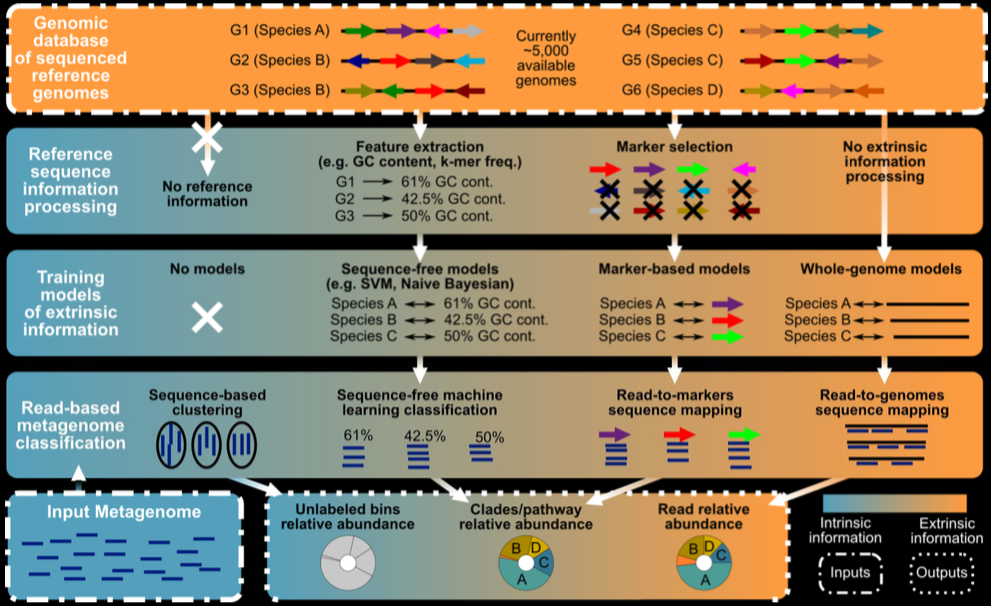
\includegraphics[width=0.95\textwidth]{taxApproaches.png}
\caption{\label{fig:taxApproaches}An overview of taxonomic profiling approaches}
\end{figure}

\vspace{3cm}

\subsection{The curatedMetagenomicData resource}

Since raw metagenomic sequencing data can be quite difficult to deal with computationally, this database stores features obtained from raw metagenomic datasets uniformly processed (MetaPhlAn or HUMAnN2) and integrated with associated metadata obtained from NCBI, papers and authors. This database is accessible and can be exploited to perform various types of analysis. (\href{https://bioconductor.org/packages/release/data/experiment/html/curatedMetagenomicData.html}{reference})

\begin{figure}[!h]
\centering
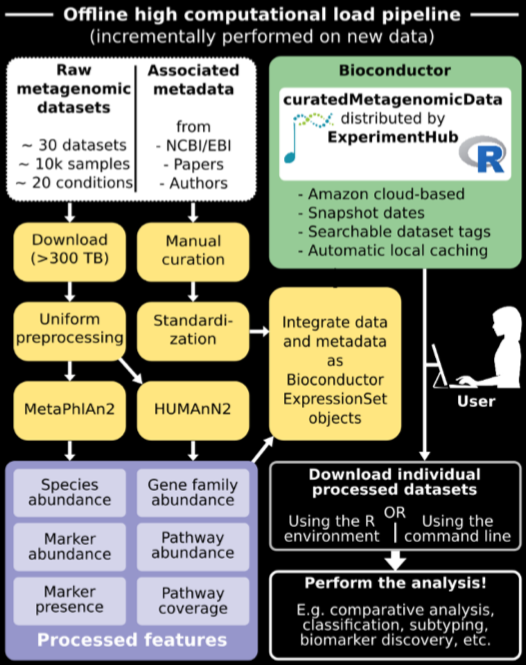
\includegraphics[width=0.4\textwidth]{curatedMetagenomicData.png}
\caption{\label{fig:curatedMetagenomicData}CuratedMetagenomicData pipeline}
\end{figure}

\subsection{The link between the gut microbiome and colorectal cancer}

\textbf{Colibactin} is a genotoxic metabolite produced by \emph{E. coli}: it causes damages to the DNA, possibly causing cancer onset. A fraction (?) of human \textbf{colorectal cancer} (CRC) cases are caused by colibactin. 

A study published by Segata’s group collected stool samples from people having a colonoscopy in Milan (\ref{fig:milanCRC}) and Turin (\ref{fig:turinCRC}). The samples were then categorized after the diagnosis provided by the colonoscopy. The aim was the identification of \textbf{biomarkers} associated with the CRC phenotype. Different results were obtained in the two cities. \\

\begin{figure}[!h]
\centering
\begin{subfigure}{.45\textwidth}
    \centering
    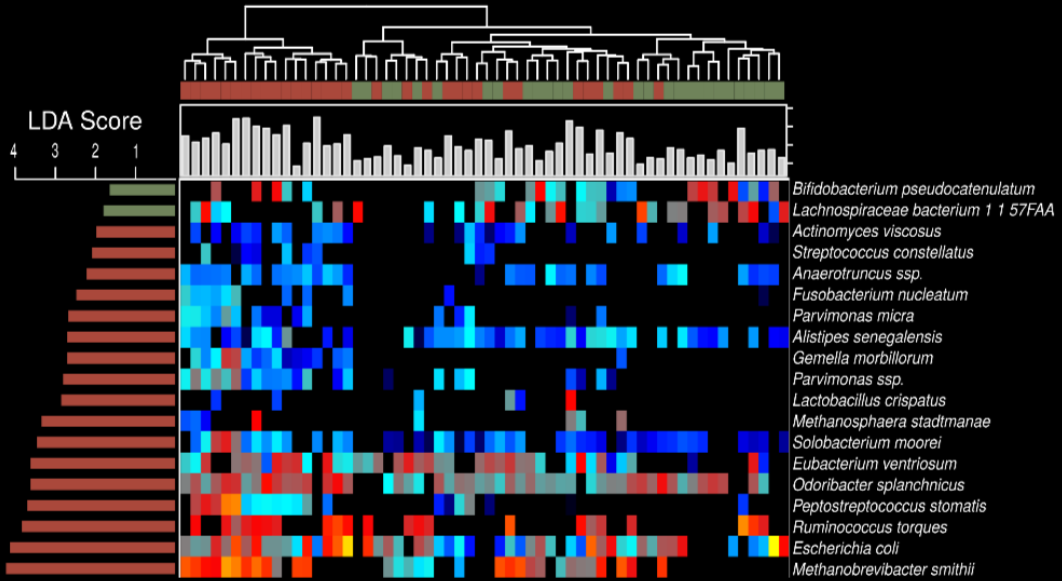
\includegraphics[width=\linewidth]{MilanCRC.png}
    \caption{\label{fig:milanCRC}Patients from Milan}
\end{subfigure}
%
\begin{subfigure}{.45\textwidth}
    \centering
    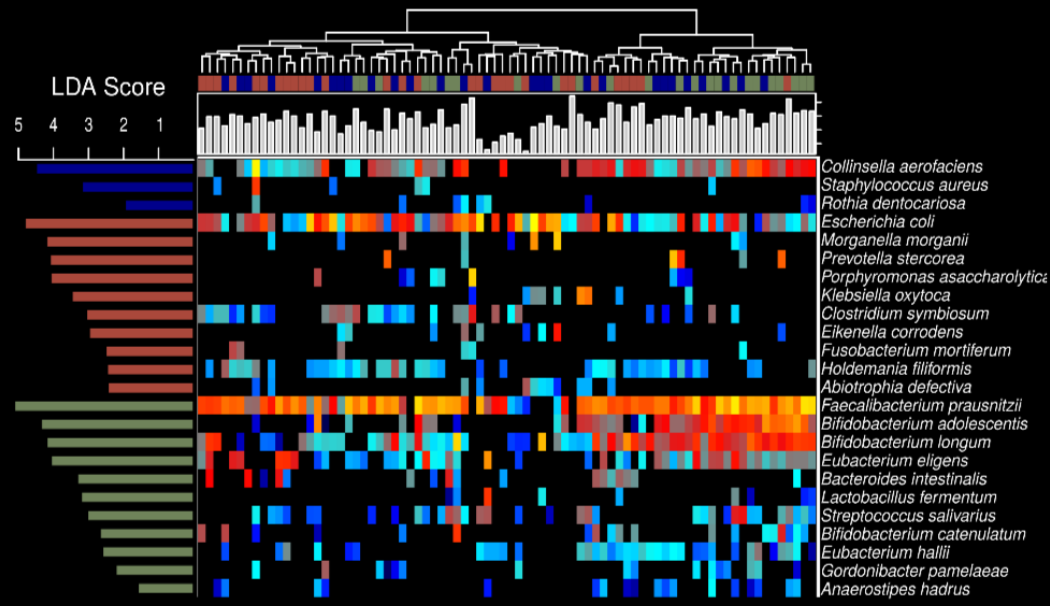
\includegraphics[width=\linewidth]{TurinCRC.png}
    \caption{\label{fig:turinCRC}Patients from Turin}
\end{subfigure}
\caption{Taxonomic profiling of gut microbiomes}
\end{figure}

Comparing this study with similar ones performed around the world (France, China, Austria, USA, Germany and Japan) some biomarkers appeared to be reproducible (\ref{fig:biomarkers}). Moreover, an accuracy around 80\% was observed when a machine learning approach (random forest) was applied on all the datasets combined and then the model was applied on a brand new one(\ref{fig:ML}). On the other hand, when each group tried the same approach on their data separately, completely different results were found for each dataset, showing that such a technique could be valid for some cases and completely useful for others. 

\begin{figure}[!h]
\centering
\begin{subfigure}{.45\textwidth}
    \centering
    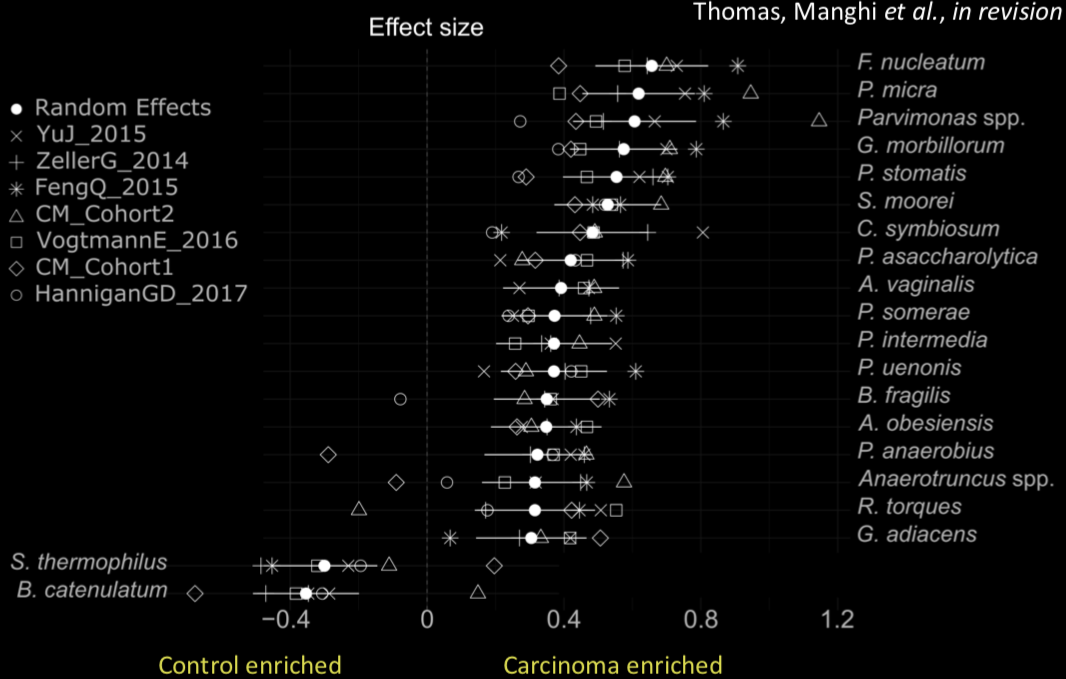
\includegraphics[width=\linewidth]{CRCbiomarkers.png}
    \caption{\label{fig:biomarkers} \emph{F. nucleatum} found to be enriched in datasets with different origins}
\end{subfigure}
%
\begin{subfigure}{.45\textwidth}
    \centering
    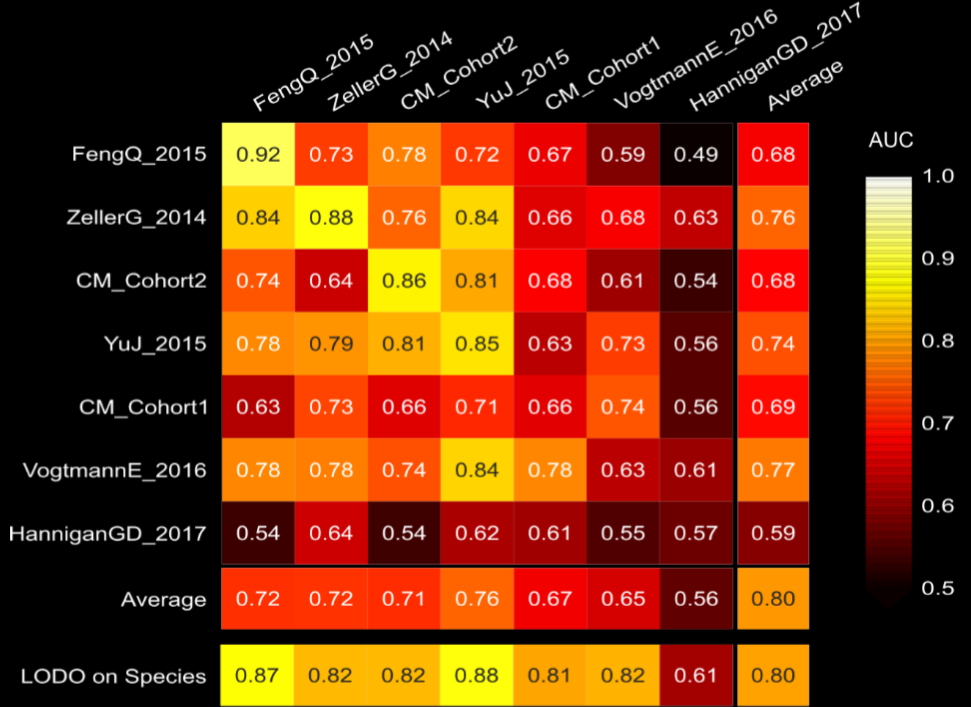
\includegraphics[width=\linewidth]{CRC_ML.png}
    \caption{\label{fig:ML}Random forest approach on all the datasets shows an accuracy of 0.80 (AUC of 1 = always right prediction, 0.5 = no prediction ability)}
\end{subfigure}
\caption{}
\end{figure}


\subsubsection{Hypothesis-driven analysis}

The \textbf{cutC} gene appears to be associated with the CRC phenotype (\ref{fig:cutC}). The problem is that it is present in several microbial species and it is unknown whether the function and the efficiency are maintained.

\begin{figure}[h]
\centering
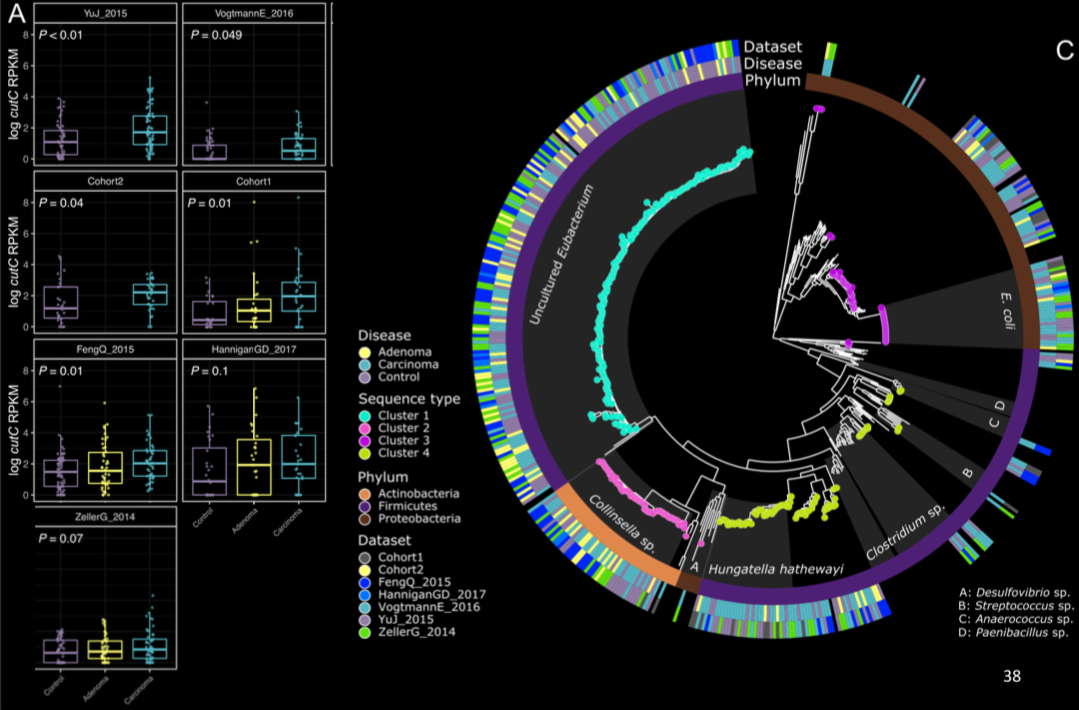
\includegraphics[width=0.5\textwidth]{cutC.png}
\caption{\label{fig:cutC}}
\end{figure}

\section{PanPhlAn: strain-level profiling}

Another tool brought to you by Segata’s crew (\href{http://segatalab.cibio.unitn.it/tools/panphlan/index.html}{reference}). \\

\textbf{PanPhlAn} is a tool for strain-level metagenomic profiling that allows to identificate gene composition of individual strains in metagenomic samples.\\ 

Challenges:
\begin{itemize}
    \item Identify the microbial strains present in the metagenome. One could also check whether a specific strain is present but the chances of finding one specific strain in a random sample are low.
    \item Discover new strains and species.
    \item Characterize the metagenome genomically.
    \item Track across samples to find the same strain and eventually prove that transmission of bacterial strains occurred among them.
\end{itemize}

The \emph{E. coli} pan genome contains about 20.000 gene-families. The goal is to find what strains are present in the metagenome and their abundances.

First all genes are grouped in \textbf{functional gene-families} (\ref{fig:pan1}). Then genes from \emph{E. coli} found in the metagenome are mapped on \emph{E. coli} reference genomes with BowTie2. The coverage is computed for each gene and then they are grouped into gene-families (\ref{fig:pan2}). Then gene-families are ranked based on their coverage. Multi-copy gene families have really high coverage, while the plot shows a plateau of single-copy gene-families. These families correspond to the strains present in the metagenome and their abundance can be deducted thanks to the base coverage of single-copy genes. 

\begin{figure}[!h]
\centering
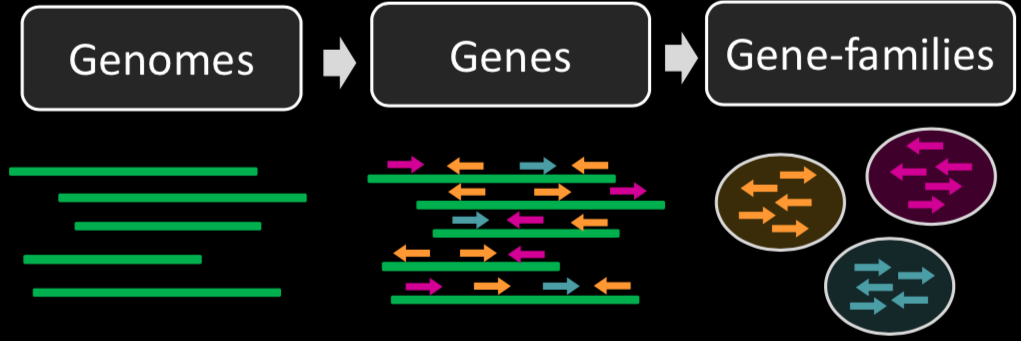
\includegraphics[width=0.9\textwidth]{panphlan1.png}
\caption{\label{fig:pan1}Genes are grouped in functional gene-families}
\end{figure}

\begin{figure}[!h]
\centering
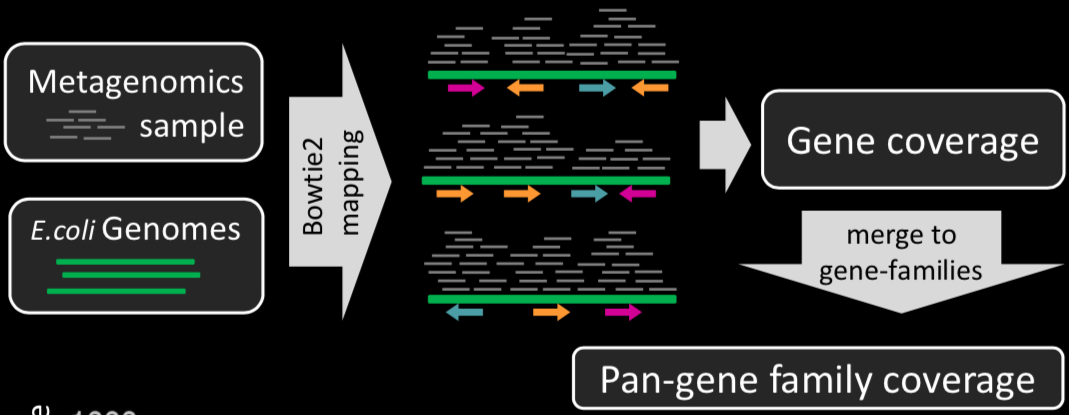
\includegraphics[width=0.9\textwidth]{panphlan2.png}
\caption{\label{fig:pan2}Mapping and subsequent coverage of gene-families}
\end{figure}

\begin{figure}[!h]
\centering
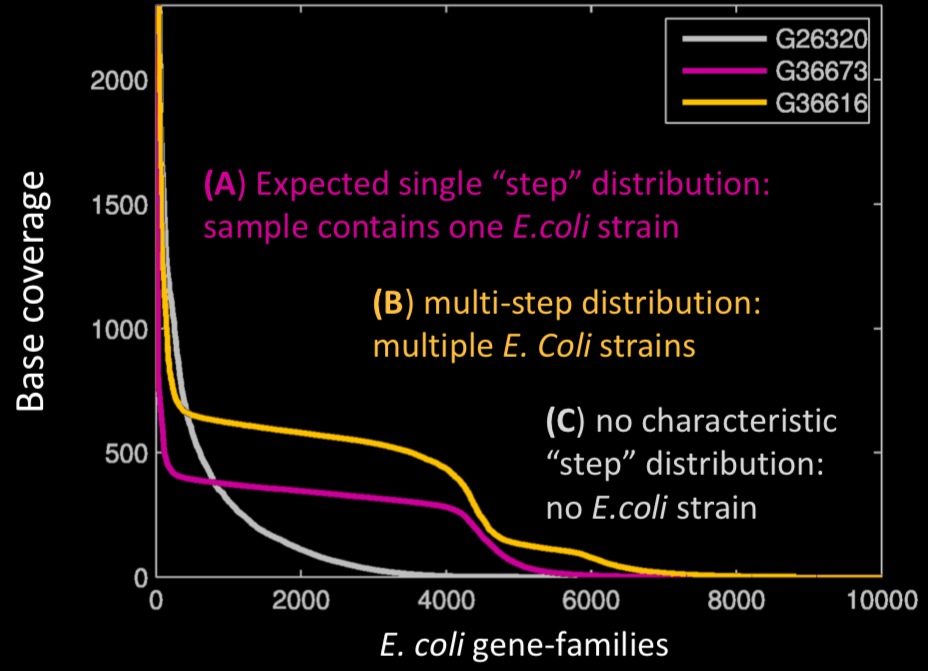
\includegraphics[width=0.6\textwidth]{Coverage.png}
\caption{\label{fig:pan3}\emph{E. coli} gene-family distribution: curve (A) shows the typical gene-families distribution: multi-copy genes with extremely high coverage, a plateau of single-copy genes and a tail of non-present gene-families. Curves like (C ) should be discarded from the analysis because they indicate that no \emph{E. coli} strain is detected in that sample.}
\end{figure}

\subsection{Investigating population genomics thanks to PanPhlAn}

\subsubsection{\emph{E. coli} population genomics with PanPhlAn}

\href{https://www.nature.com/articles/nmeth.3802}{\emph{Scholz, M., Ward, D., Pasolli, E. et al. Strain-level microbial epidemiology and population genomics from shotgun metagenomics. Nat Methods 13, 435–438 (2016).}} \\

Figure \ref{fig:Ecoli1} shows the \emph{E. coli} profiling of 1478 shotgun metagenomes carried out with PanPhlAn. Each column is either an \emph{E. coli} strain obtained via shotgun metagenomics or a reference strain and the columns correspond to the gene-families that can be absent or present in each strain. The strains are then clustered (\ref{fig:Ecoli2}) based on which gene-families are present in order to study the population genomics: in this case we can see that the strains isolated from the German \emph{E. coli} outbreak cluster together, while other strains are present in several different areas of the world. 

\begin{figure}[!h]
\centering
\begin{subfigure}{.49\textwidth}
    \centering
    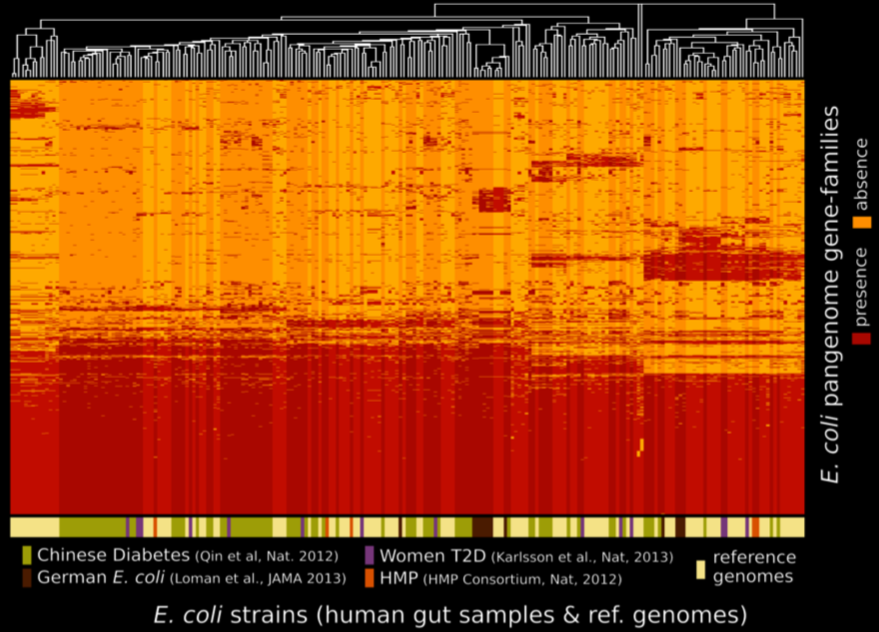
\includegraphics[width=\linewidth]{Ecoli1.png}
    \caption{\label{fig:Ecoli1}}
\end{subfigure}
%
\begin{subfigure}{.49\textwidth}
    \centering
    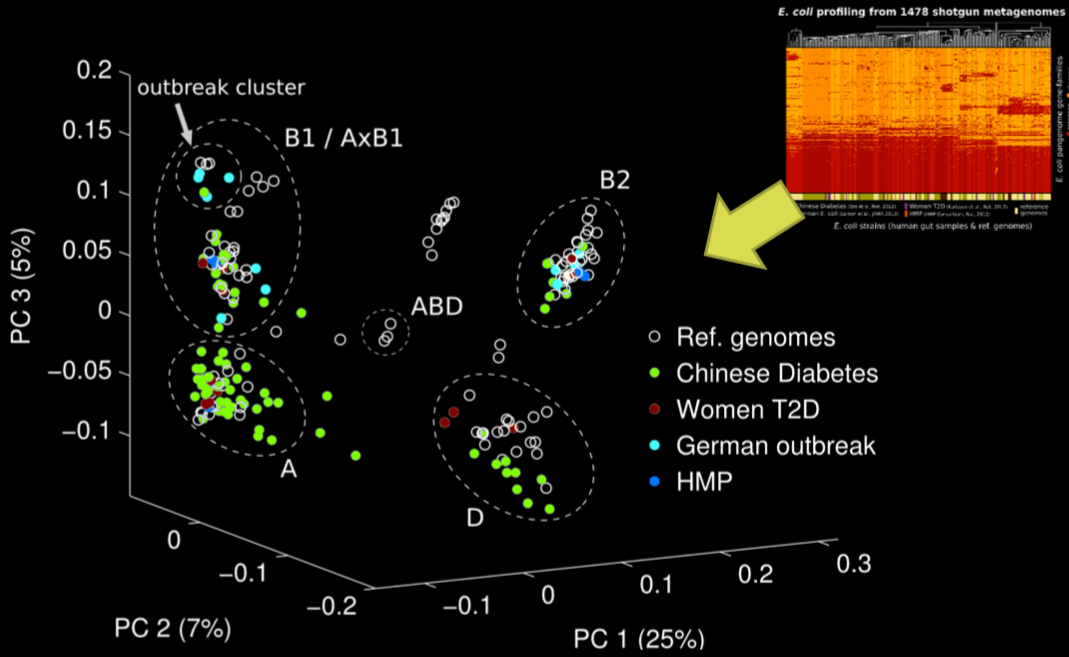
\includegraphics[width=\linewidth]{Ecoli2.png}
    \caption{\label{fig:Ecoli2}}
\end{subfigure}
\caption{\emph{E.coli} population genomics with PanPhlAn}
\end{figure}

\vspace{2cm}

\subsubsection{PanPhlAn on \emph{Eubacterium rectale}}

Thanks to PanPhlAn, it was possible to identify many subtypes of \emph{E.rectale} even though only one reference genome was available at the time (\ref{fig:Erec}).

\begin{figure}[!h]
\centering
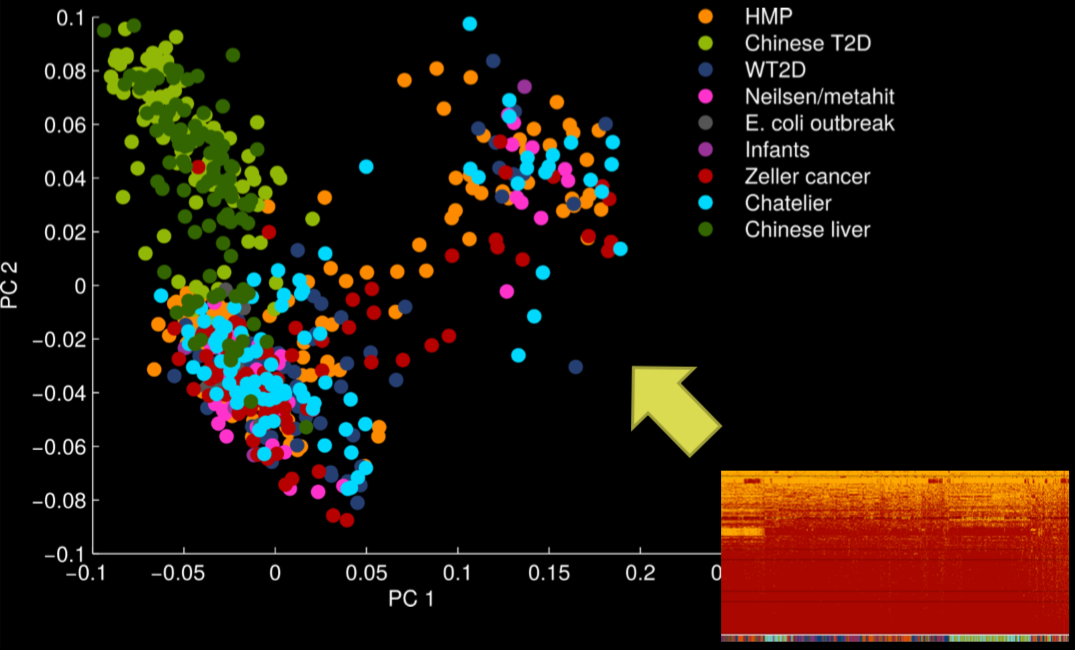
\includegraphics[width=0.6\textwidth]{Erectale.png}
\caption{\label{fig:Erec} PanPhlAn on \emph{Eubacterium rectale}}
\end{figure}

\subsubsection{The infant gut microbiome in disease}

\href{https://www.cell.com/cell-reports/pdf/S2211-1247(16)30256-X.pdf}{\emph{Ward et al. Cell Reports 2016}} \\

\textbf{Necrotizing Enterocolitis} (NEC) is a devastating disease that affects mostly the intestines of premature infants. This study took samples from a cohort of 173 infants, 151 of them were preterm and 30 of them had NEC. They obtained 460 shotgun metagenomic samples and 284 shotgun metatranscriptomic samples, all of which were coupled with clinical data of the patients. The heatmap shows MetaPhlAn profiling of different bacterial species for all the samples: about 20\% of the patients have a high \emph{E. coli} predominance (\ref{fig:nec1}: yellow circle). PanPhlAn was employed to investigate the \emph{E. coli} strains found in these patients: of the 4 identified clades, only 2 are associated with NEC (\ref{fig:nec2}).

\begin{figure}[!h]
\centering
\begin{subfigure}{.45\textwidth}
    \centering
    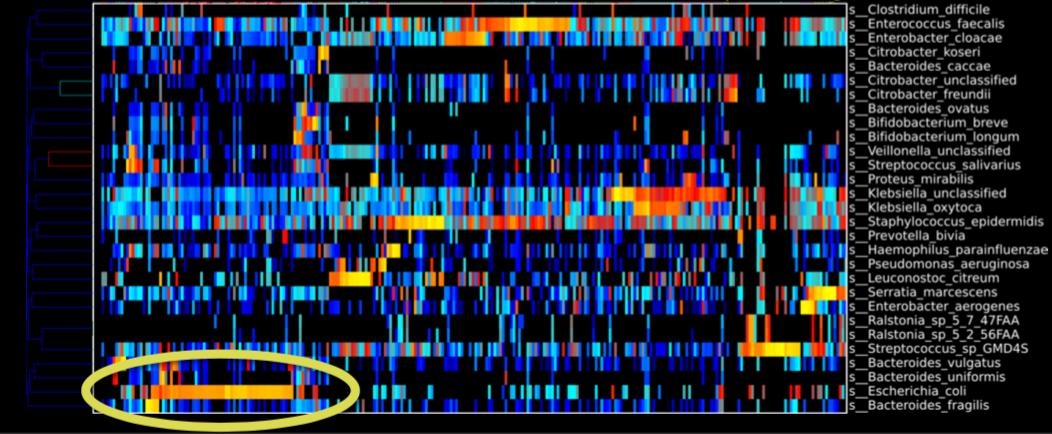
\includegraphics[width=\linewidth]{nec1.png}
    \caption{\label{fig:nec1}MetaPhlAn2 profiling of the cohort of infants}
\end{subfigure}
%
\begin{subfigure}{.45\textwidth}
    \centering
    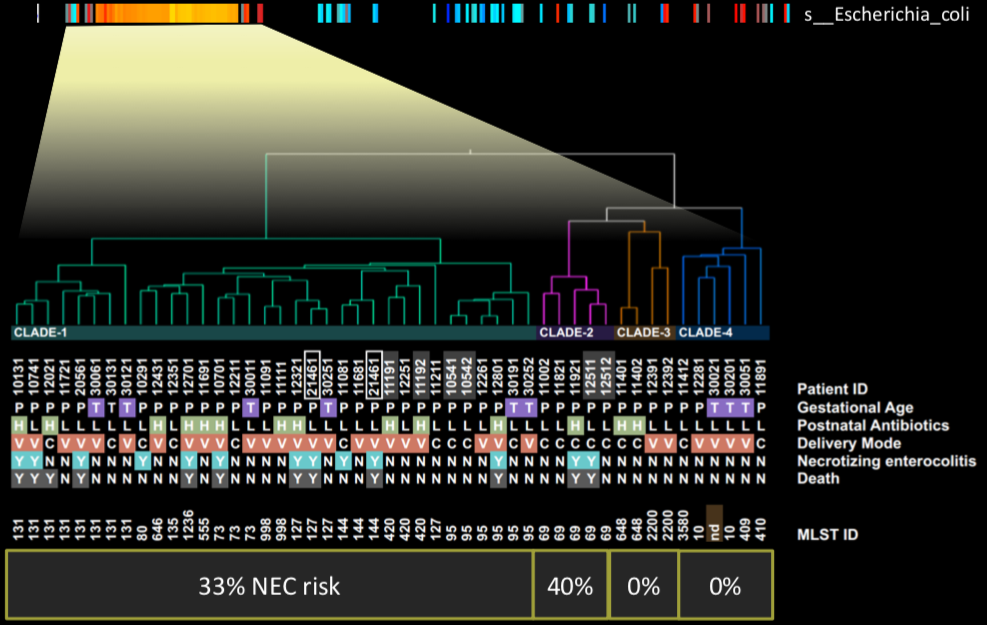
\includegraphics[width=\linewidth]{nec2.png}
    \caption{\label{fig:nec2}PanPhlAn to resolve NEC-assocated E. coli diversity}
\end{subfigure}
\caption{The infant gut microbiome in disease}
\end{figure}

\subsection{StrainPhlAn: a complementary approach}

As usual, tool by Segata and friends( \href{http://segatalab.cibio.unitn.it/tools/strainphlan/index.html}{reference}) \\

The idea is to base the classification on the \textbf{genetic variance} of core genomes: look for unique combinations of \textbf{SNPs} in genes that are always present and analyze their variance to find some SNPs with a variance different from the others that could characterize a new strain.

\textbf{StrainPhlAn} exploits MetaPlAn to compute species-level abundances thanks to species-specific markers and then aligns the marker genes present in the samples to find the SNPs. The SNPs are then analyzed to build a phylogenetic tree.

This approach can be applied to many different species. or \emph{E. rectale} it seems to have a higher resolution compared to the previous approach.

\begin{figure}[!h]
\centering
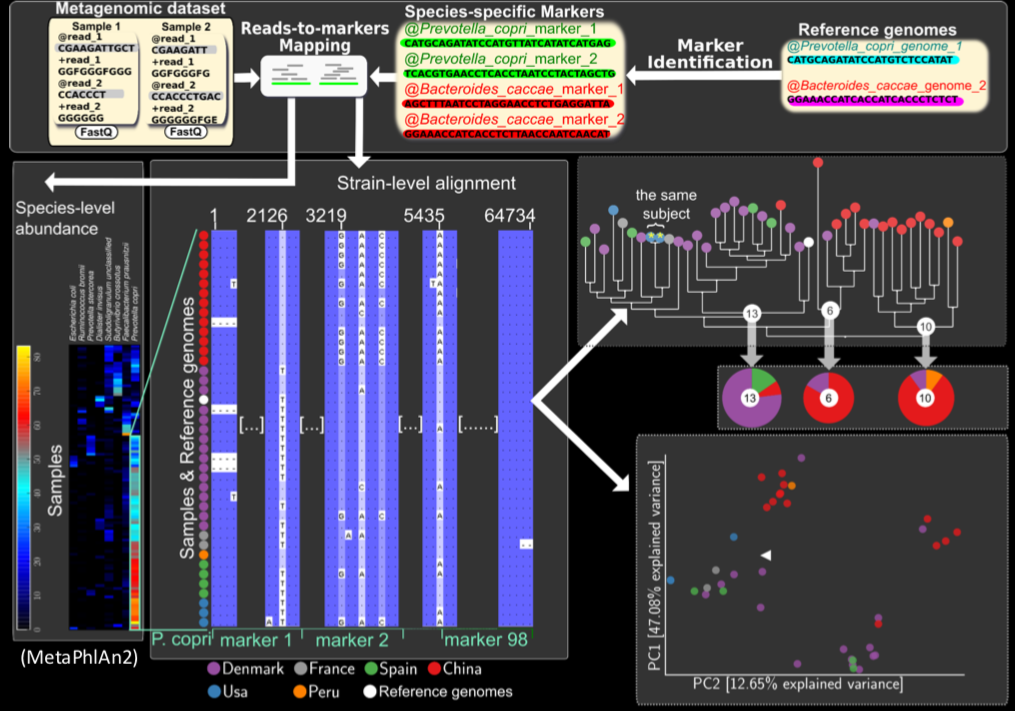
\includegraphics[width=0.9\textwidth]{StrainPhlAn.png}
\caption{\label{fig:strainphlan}StrainPhlAn pipeline}
\end{figure}

\subsection{StrainPhlAn applications}

\subsubsection{The stability of strains in the human gut}

\begin{figure}[!h]
\centering
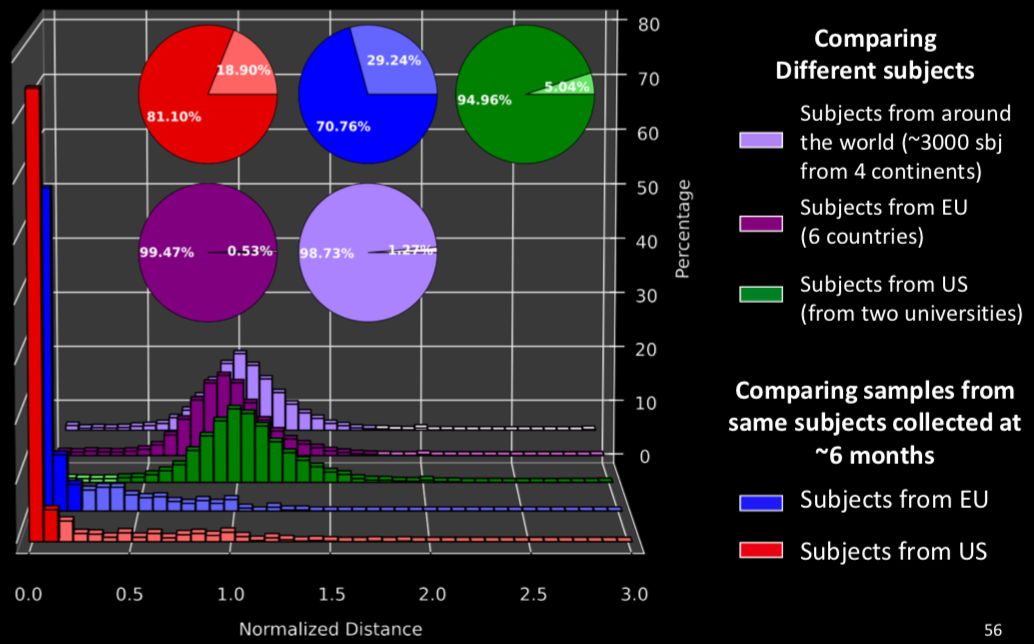
\includegraphics[width=0.8\textwidth]{strainGut.png}
\caption{\label{fig:gut}The stability of strains in the human gut}
\end{figure}

This study analyzes samples of the human gut microbiome obtained from different continents. The barplots (\ref{fig:gut}) show the distances measured between results of SNPs analysis in different regions around the world. There are almost no pairs with zero or low distance and the results do not change if only subjects from the EU or US are considered.
On the other hand, the red and blue barplots (\ref{fig:gut}) show that comparing the SNPs of samples coming from the same individual but collected 6 months apart they show great similarity. This indicates that there is some stability in the human gut microbiome: usually the strains present in one’s gut microbiome tend to remain almost the same. Nevertheless, changes of diet or other habits can bring variations in their abundances.

\subsubsection{Identification of subspecies}

\begin{figure}[!h]
\centering
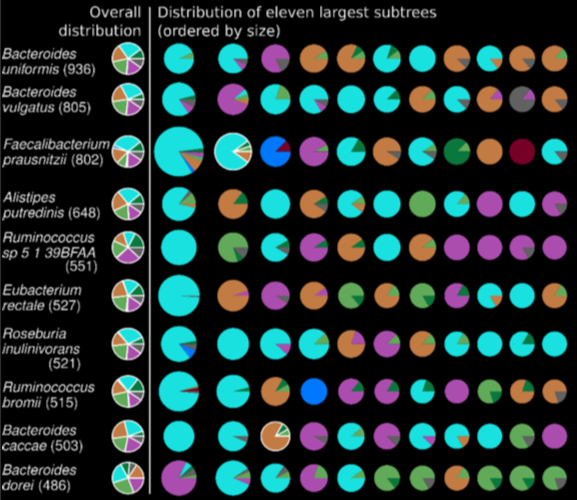
\includegraphics[width=0.5\textwidth]{strainGeo.png}
\caption{\label{fig:geo}Association of sub-species structures with geography}
\end{figure}

Some bacteria are strongly represented in the human population’s microbiomes and their presence is detected in all continents. Everything changes when looking at \textbf{subspecies}: some of them are highly region-specific. 
Un Figure \ref{fig:geo}, each color indicates a different country: it is clear that when looking at subspecies of these common microbes, they are mostly associated with only one country/continent.

\subsection{Uncharacterized species}

A great amount of information about the human is still unknown:
\begin{itemize}
    \item \textbf{Functional unknowns}: genes for which we still do not know the function because they do not match any functional database.
    \item \textbf{Unknown species/strains}: genes not matching any of the known reference genomes.
    \item \textbf{Undetected unknowns}: things we do not know and were not even observed yet.
\end{itemize}

\textbf{Westernized} metagenomes are more characterized than non-westernized ones: \\

\href{https://www.sciencedirect.com/science/article/pii/S0092867419300017}{\emph{Pasolli, Edoardo et al. “Extensive Unexplored Human Microbiome Diversity Revealed by Over 150,000 Genomes from Metagenomes Spanning Age, Geography, and Lifestyle.” Cell vol. 176,3 (2019}}\\

This study performed a large-scale metagenomic assembly on data from uncharacterized regions of the world.
They were able to reconstruct ~70.000 high quality genomes and ~85.000 medium-quality ones (with ~50\% completeness)\\

\textbf{Workflow} (\ref{fig:workflow2}):
\begin{itemize}
    \item Assembly of the reads into contigs
    \item Binning of contigs into putative genomes (MAGs = Metagenome-Assembled Genomes)
    \item Quality control
\end{itemize}

The MAGs are then clustered (also thanks to reference genomes) in \textbf{Species-level Genome Bins} (SGBs) by measuring the distance scores between couples of putative genomes. SGBs are divided into known \textbf{kSGBs} (if they contain at least one reference genome), unknown \textbf{uSGBs} (they are not identified but can be used to detect novel marker genes) and non-human SGBs. \\

\begin{figure}[h]
\centering
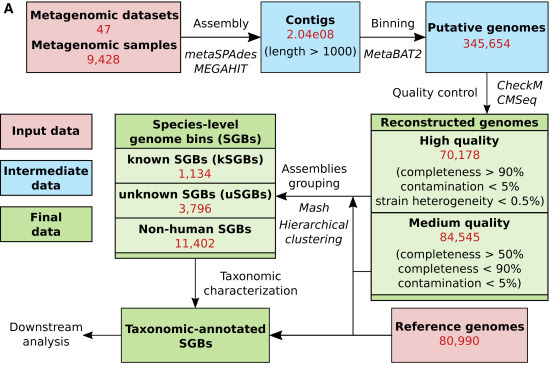
\includegraphics[width=0.9\textwidth]{workflow2.jpg}
\caption{\label{fig:workflow2}Workflow of large-scale metagenomic assembly}
\end{figure}

In this study they also characterized a new bacterium: the \textbf{Cibiobacter} (this is how they named it but sadly they had to change). Interesting fact: Madagascar-associated strains of Cibiobacter uniquely possess the trp operon for tryptophan metabolism.

\subsection{Applications of strain-level metagenomic profiling}

\subsubsection{\emph{E.rectale} refined population genomics}

\href{https://genomebiology.biomedcentral.com/articles/10.1186/s13059-020-02042-y}{\emph{Karcher, N., Pasolli, E., Asnicar, F. et al. Analysis of 1321 Eubacterium rectale genomes from metagenomes uncovers complex phylogeographic population structure and subspecies functional adaptations. Genome Biol 21, 138 (2020)}}\\

\begin{figure}[!h]
\centering
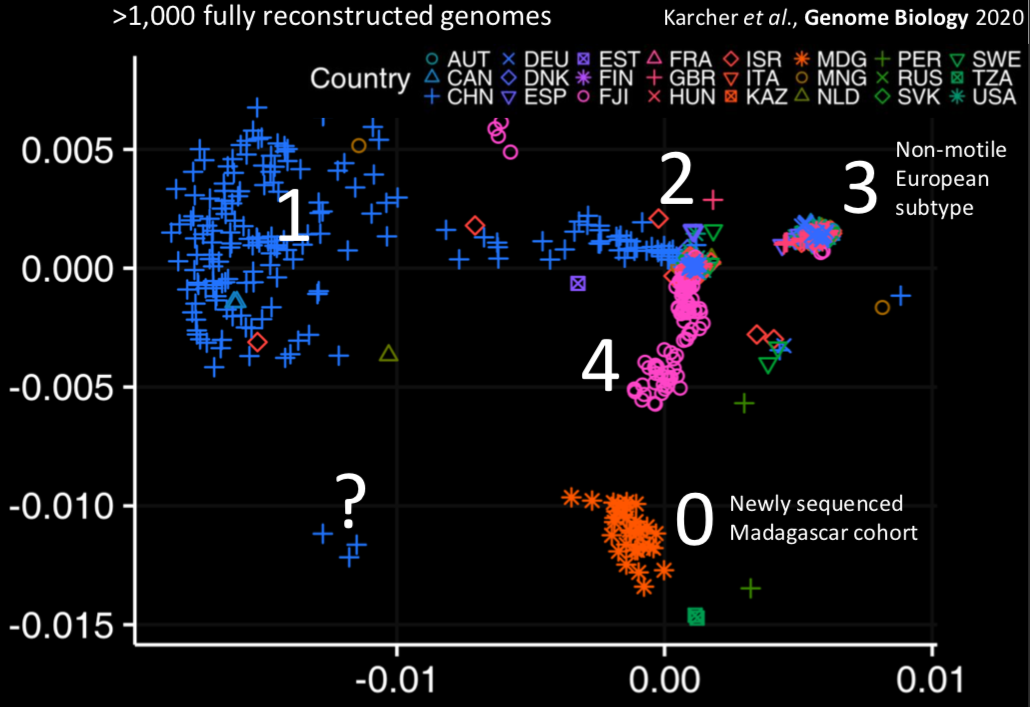
\includegraphics[width=0.8\textwidth]{Erec2.png}
\caption{\label{fig:Erec2}\emph{E.rectale} refined population genomics}
\end{figure}

Thanks to the advancements brought by strain-level metagenomic profiling, a new subtype of \emph{E. rectale} was discovered. Subtype 3 lacks the operon coding for motility and other genes that become useless for the bacteria if it is not motile. On the other hand, they present more copies of the \textbf{CAZy} genes: these are involved in metabolism and are required by non-motile bacteria in order to be more efficient in the exploitation of carbon sources since they cannot move to reach them.

\subsubsection{\emph{Prevotella copri} is strongly lifestyle-associated}

\href{https://www.sciencedirect.com/science/article/pii/S1931312819304275}{\emph{Tett, Adrian et al. “The Prevotella copri Complex Comprises Four Distinct Clades Underrepresented in Westernized Populations.” Cell host $\&$ microbe vol. 26,5 (2019)}}\\

\begin{figure}[!h]
\centering
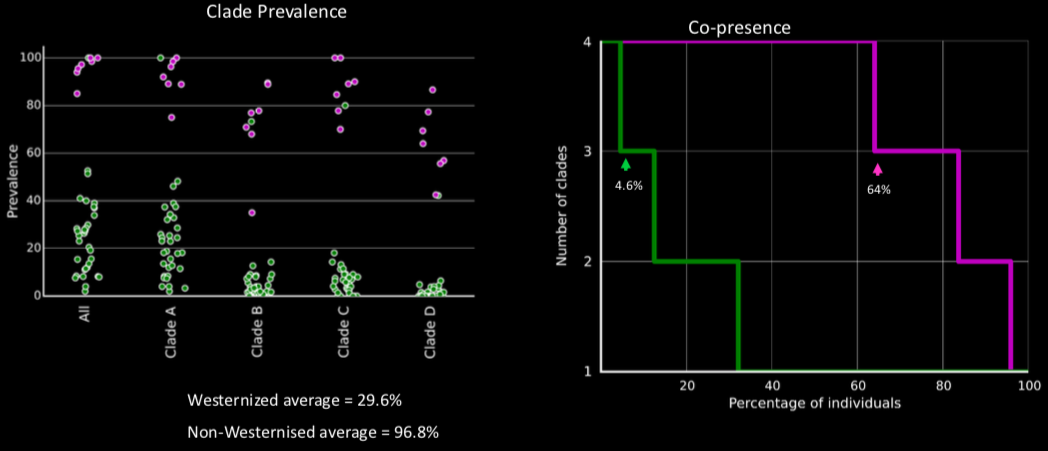
\includegraphics[width=0.8\textwidth]{Prevotella.png}
\caption{\label{fig:prevotella}\emph{Prevotella copri} is strongly (Western) life-style associated}
\end{figure}

\emph{P. copri} is a frequent bacterium in the gut microbiome and it tends to be an on/off one: if it is present, it is often dominant.
4 \emph{P. copri} clades with the ability of degrading complex fibers were found. They are called clades just because it is not yet confirmed that they can be considered as new strains. 
The interesting part is that westernized populations are associated with a lower prevalence of these clades and with a lower probability of presenting all the 4 clades together (\ref{fig:prevotella}). This is probably caused by our diet: westernized populations tend to eat less complex fibers than non-westernized ones.
This was confirmed by the analysis of the microbiome found in Otzi (3.300 BC) and some ancient Mexican coprolites (nice term to say cacca mummificata) (600-1300 AD). The \emph{P. copri} clades were found in these samples, indicating that we are possibly losing \emph{P. copri} in the westernized populations.

\subsubsection{Identification of \emph{Akkermansia} candidate subspecies}

\href{https://genomebiology.biomedcentral.com/articles/10.1186/s13059-021-02427-7}{\emph{Karcher, N., Nigro, E., Punčochář, M. et al. Genomic diversity and ecology of human-associated \emph{Akkermansia} species in the gut microbiome revealed by extensive metagenomic assembly. Genome Biol 22, 209 (2021)}}\\

Only two subspecies of \emph{Akkermansia} have been described and characterized so far: \emph{A. muciniphila} and \emph{A. glycaniphila}. In this paper, they used PhyloPhlAn3 (Segata’s tool for phylogenetic analysis) to identify 4 MAGs that are candidate \emph{Akkermansia} species. 
Moreover, they observed that these candidate \emph{Akkermansia} species are mutually exclusive for what concerns hosts: they were rarely found coexisting in the same sample. They also appear to have different associations in respect to \emph{A. muciniphila}: one is associated with decreased host body mass index (BMI) but the others are not (\ref{fig:akk}).

\begin{figure}[!h]
\centering
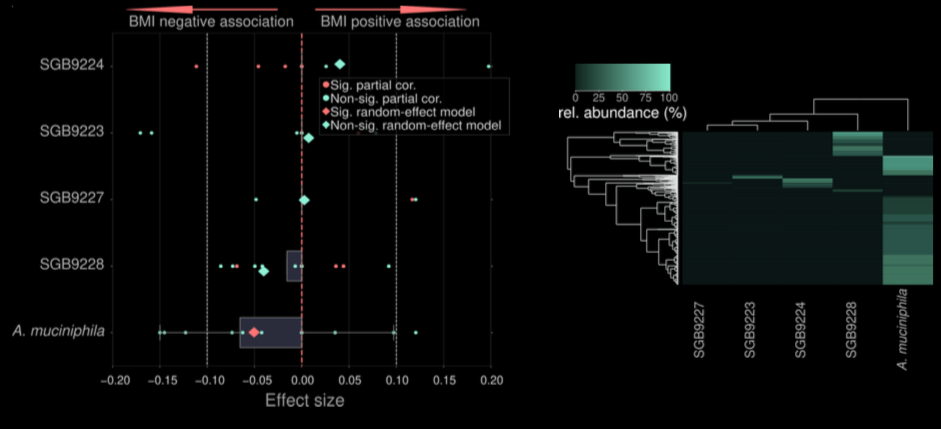
\includegraphics[width=0.8\textwidth]{akkermansia.png}
\caption{\label{fig:akk}Distinct associations and co-exclusion for the \emph{Akkermansia} (candidate) species}
\end{figure}

They also identified putative bacteriophages with spacer hits from \emph{Akkermansia} candidate species and found that viral detectability correlates strongly with the relative abundance of the \emph{Akkermansia} candidate species, suggesting an intimate ecological interplay.

Analyzing \emph{A. muciniphila} subspecies, they determined that these are host-specific: some are found only in mice and some only in humans.

\subsubsection{An example of eukaryotic microorganism: \emph{Blastocystis}}

\href{https://www.nature.com/articles/ismej2017139}{\emph{Beghini, Francesco et al. “Large-scale comparative metagenomics of \emph{Blastocystis}, a common member of the human gut microbiome.” The ISME journal vol. 11,12 (2017)}}\\

They developed a pipeline to detect \emph{Blastocystis} subtypes and applied it on 12 large datasets composed of 1689 subjects of different geographic origin, disease status and lifestyle. 

They confirmed that \emph{Blastocystis} is a component of the healthy gut microbiome and found a higher prevalence in non-westernized individuals. Moreover, they were able to construct and functionally profile 43 new \emph{Blastocystis} genomes.

A strong association of specific microbial communities with \emph{Blastocystis} was confirmed by the high predictability of the microorganism colonization based on the species-level composition of the microbiome.   

\subsubsection{Bacteriophages profiling}

Just know that it is possible.

\begin{figure}[!h]
\centering
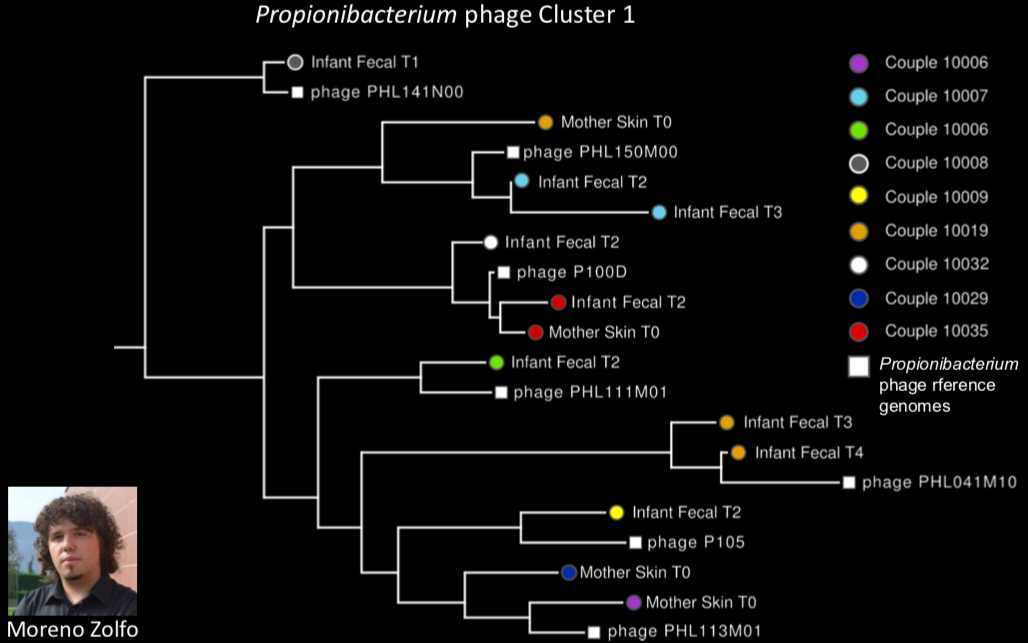
\includegraphics[width=0.8\textwidth]{phages.png}
\caption{\label{fig:phages}\emph{Propionibacterium} phage Cluster 1}
\end{figure}

\subsection{HUMAnN2: Functional profiling}

The task of mapping nucleotide sequences to proteins (that can be done by blastX on a smaller scale) is important but computationally challenging. 
Multiple bacteria can be responsible for the same function in the microbiome. Thanks to this redundancy, functions are more conserved than bacterial prevalence: the abundance of a bacteria can vary but its function remains efficient because another microbe supplies it.
For functional profiling, the idea is to reduce the reference dataset by mapping the genes only across proteins that we know are present in the bacteria found in the sample. Then the remaining unclassified reads can be mapped to a comprehensive protein database \ref{fig:human2}.
\href{https://www.nature.com/articles/s41592-018-0176-y}{HUMAnN2} performs species-level functional profiling of metagenomes and metatranscriptomes.

\begin{figure}[!h]
\centering
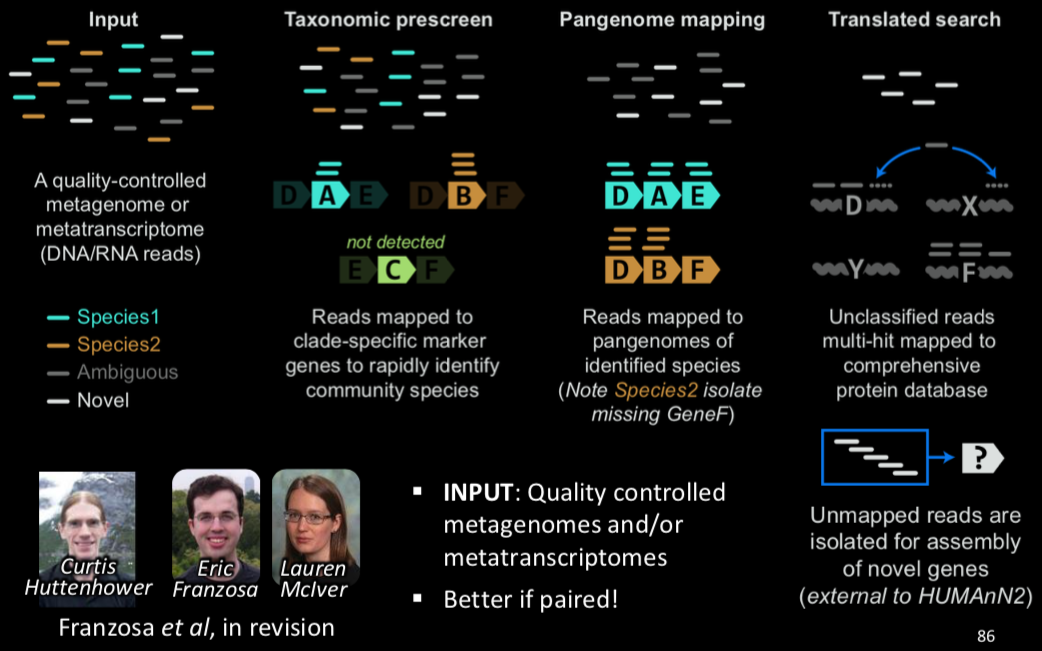
\includegraphics[width=0.8\textwidth]{human2.png}
\caption{\label{fig:human2}HUMAnN2 workflow}
\end{figure}
